\chapter{Results}

\begin{figure}[h]
    \centering
    \begin{subfigure}[h]{1.0\textwidth}
        \centering
        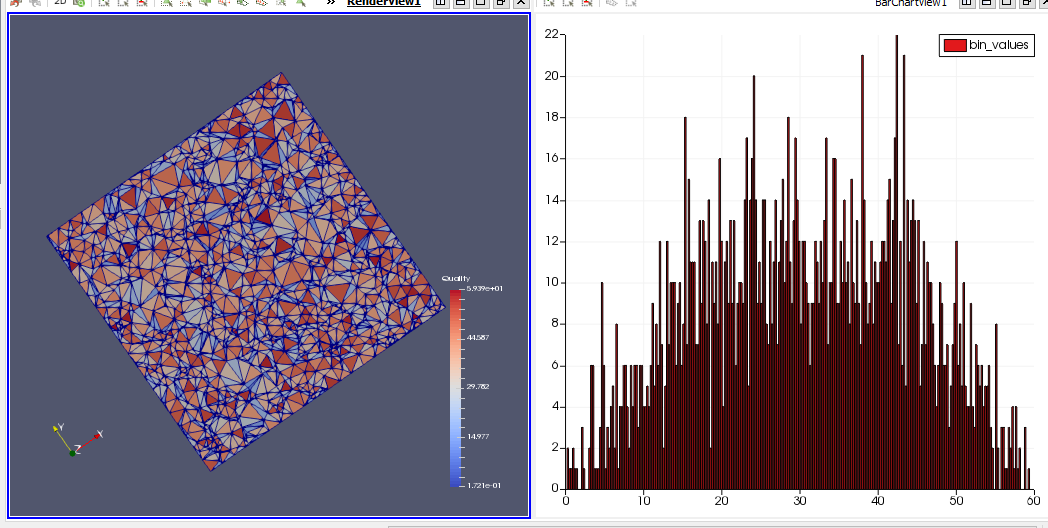
\includegraphics[width=\textwidth]{images/original_1000.png}
        \caption{Original}
    \end{subfigure}
    \vspace{0.5 cm}
 
    \begin{subfigure}[h]{1.0\textwidth}
        \centering
        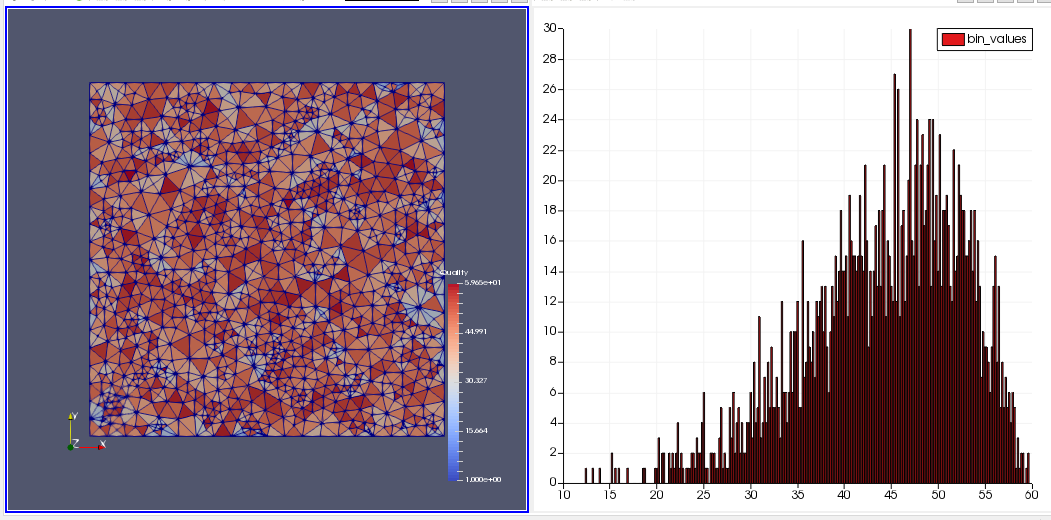
\includegraphics[width=\textwidth]{images/laplacian_no_flips_1000.png}
        \caption{Smart Laplacian without flips}
    \end{subfigure}
    \vspace{0.5 cm}
 
    \begin{subfigure}[h]{1.0\textwidth}
        \centering
        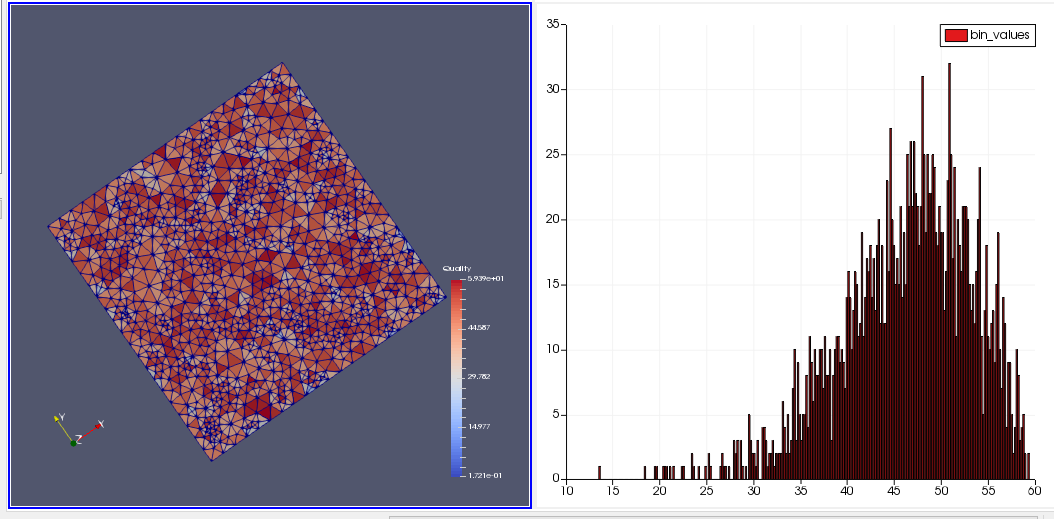
\includegraphics[width=\textwidth]{images/laplacian_1000.png}
        \caption{Smart Laplacian with flips}
    \end{subfigure}
	\vspace{0.5 cm}
\end{figure}

\begin{figure}[h]
	\ContinuedFloat
    \centering
   	\begin{subfigure}[h]{1.0\textwidth}
        \centering
        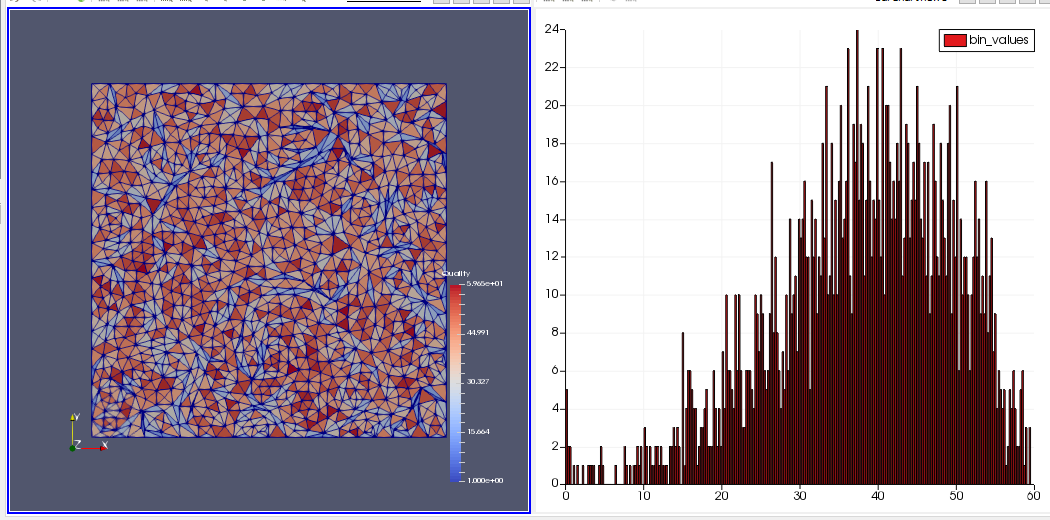
\includegraphics[width=\textwidth]{images/aspect_ratio_no_flips_1000.png}
        \caption{Aspect Ratio Based without flips}
    \end{subfigure}
	\vspace{0.5 cm}
	    
    \begin{subfigure}[h]{1.0\textwidth}
        \centering
        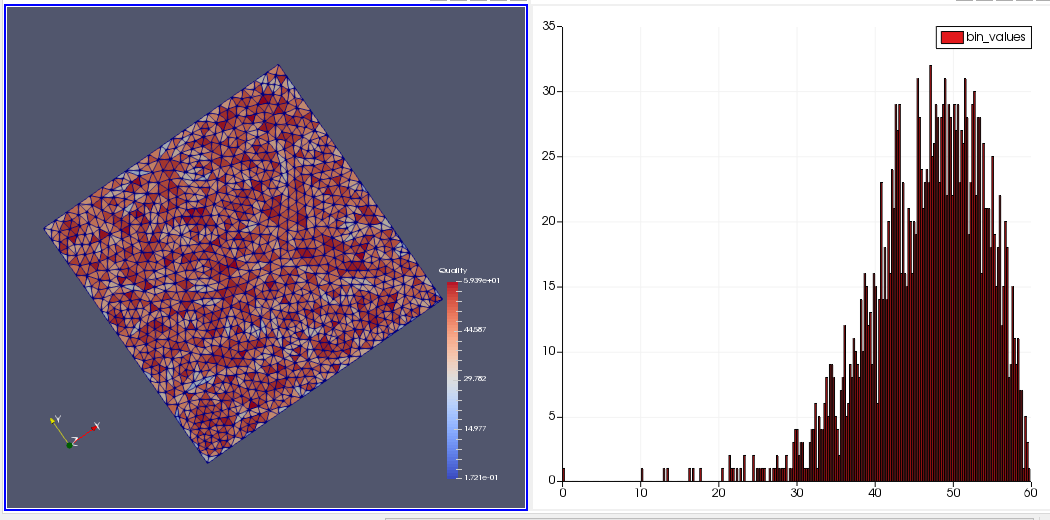
\includegraphics[width=\textwidth]{images/aspect_ratio_1000.png}
        \caption{Aspect Ratio Based with flips}    
    \end{subfigure}	  	
    \caption{Delaunay mesh of square having 1000 vertices}
    \label{fig:points_1000}
\end{figure}